%%%%%%%%%%%%%%%%%%%%%%%%%%%%%
% Dissertation Thesis by    %
%        Wesley Honeycutt   %
%                           %
% Designed for the PhD re-  %
% quirements at Oklahoma    %
% State University as of    %
% Spring 2017.              %
%%%%%%%%%%%%%%%%%%%%%%%%%%%%%
% This is the root document %
% This is where you should  %
% put any LaTeX packages,   %
% options, and chapters.    %
% The class for this LaTeX  %
% document is found in the  %
% okstate.cls file included %
% in the directory.  The    %
% directories for this pro- %
% ject are arranged in the  %
% following heirachy:       %
%                           %
%  chapters\                %
%  images\                  %
%  #rootDissertation.tex    %
%  okstate.cls              %
%  okstate.clo              %
%%%%%%%%%%%%%%%%%%%%%%%%%%%%%
% The last update to class  %
% files and heirachy was on %
%                           %
%       2017-MAR-07         %
%%%%%%%%%%%%%%%%%%%%%%%%%%%%%

\documentclass[12pt]{okstate}
%\documentclass[12pt,demo]{okstate} %Use this class switch to ignore pictures.  This is useful to avoid long compilation times with graphics heavy dissertations.

% Packages Required for this document or the OSU style
\usepackage{fullpage}
\usepackage{graphicx}
\usepackage{natbib} 
	\bibliographystyle{unsrt}
\usepackage{titlesec}
\usepackage{setspace}

% These packages are what I personally use which are recommended for others
%\usepackage{amsmath} % Makes pretty equations
%\usepackage[version=3]{mhchem} % Makes pretty chemistry
%\usepackage{url} % Prevents urls from breaking in the 
%\usepackage{placeins} % Allows the use of \FloatBarrier when you have many figures
%\usepackage{threeparttable} % Allows use of more complicated tables
%\usepackage{subcaption} % ???
%\usepackage{pdfpages} % Allows you to insert PDF images as pages/figures
%\usepackage{listings} % Allows you to insert code, markdown
%\usepackage{multirow} % ????
%\usepackage[super]{nth} % Useful for ordinal numbers
%\usepackage{siunitx} % Useful for correct use of SI units
%\usepackage{soul} % Useful for highlighting and editing with \hl

% This recommended package always goes LAST in your list.  Possibly magic.
\usepackage{microtype}

\graphicspath{ {images/} } %this removes clutter from the root folder








%% Author's personal definitions go here
\newcommand{\angstrom}{\textup{ \AA}} % siunitx doesn't support angstroms
\newcommand{\degree}{$^{\circ}$} % I used this in my old tables, possibly can be replaced by siunitx options, but I'm too lazy to deal with that right now.




%%% This is required formatting for OSU dissertations.  Do not touch.
%Settings for the Chapter Titles
%Requires titlesec package
\titleformat{\chapter}[display]
	{\normalfont\filcenter}
	{\vspace{6.0225pc}%
	\centering%
	\scshape \chaptertitlename~\thechapter%
	\vspace{3.01125pc}%
	}{3.01125pc}{}

% the date
\date{\today}










%%%%%%% Dissertation Specific Fields  %%%%%

% No symbols, formulas, superscripts, or Greek letters are allowed in your title.
 \title{Dissertation Title Goes Here}
 
% Your name.
\author{Pistol Pete}

% The month and year the degree will be officially conferred
\degreeyear{May 20xx}

% The full (unabbreviated) name of the degree
\degreetitle{Doctor of Philosophy}

% The field your degree will be in
\field{Mathematics}

%%%%%%% Your Committee Goes Here      %%%%%
% To match OSU's style, make sure to use the same title for each committee member if possible.  e.g. if you call one Dr., they all get called Dr. and if you call one Prof., they all get called Prof.
%% This class only supports a fixed number of committee members right now. - WTH 2/22/17
%% This class only does not support co-chairs right now. - WTH 2/22/17

% Your advisor
\comchair{Dr. Robert Barker}

% Your other committee members
% Use alphabetical order for these
\comfirst{Dr. Henry E. Alvord}
\comsecond{Dr. Edmund D. Murdaugh}
\comthird{Dr. George E. Morrow}

% Your outside committee member
\comout{Dr. Angelo C. Scott}

%%%%%%% Your Abstract Goes Here       %%%%%

 \abstract{This abstract is abstract. This abstract is abstract. This abstract is abstract. This abstract is abstract. This abstract is abstract. This abstract is abstract. This abstract is abstract. This abstract is abstract. This abstract is abstract. This abstract is abstract. This abstract is abstract. This abstract is abstract. This abstract is abstract. This abstract is abstract. This abstract is abstract. }
 
 %%%%%%% Your Acknowledgements Go Here %%%%%
 
\acknow{Thank you to people, things, and places. Without them this thesis would be a meaningless arrangement of ink dots.}












% The actual document
\begin{document} 
	
	%This makes the titles and required pages.
     
 %% START THE FRONTMATTER
 %% You should not have to touch this much to make it work right.
 %
 \begin{frontmatter}
 	
 	%% TITLE PAGES
 	%
 	%  This command generates the title, copyright, and signature pages.
 	%
 	\makefrontmatter 
 	\tableofcontents
 	\listoffigures  % Uncomment if you have any figures
 	\listoftables   % Uncomment if you have any tables
 	
 	
 	%This is a relic from the Uark version and UCSD version that things were borrowed from.
 	%If list of tables or figures is used with nothing after it before \end{frontmatter}, as is the OSU style, the last list will begin arabic numbering. Placing newpage strangely does not produce a blank page, but fixes the problem.
 	\newpage
 
 	
 \end{frontmatter}


	\chapter{Introduction}
	\label{chap:1}
	Welcome to the \LaTeX template for your dissertation at Oklahoma State University.  The words in here will show off some of the things built in to the template.

\section{An Introduction to Introductions}

There are lots of things you can do with this template.  I'm sure you have spent too much time slaving away over your research, so the WYSIWYW interface will help you focus on the content of your dissertation.

\subsection{Citing Sources}

The citations for this template are stored in the ``thesis.bib'' file.  The bibliography format in the ``\#rootDissertation.tex'' file is set to organize things by when they show up in the paper.  Here is a paper I cited in my dissertation~\cite{arrhenius_xxxi._1896}.

The current setup places all of your references at the end of the dissertation.  If you want to include a list of references at the end of each chapter, you should make a new ``*.bib'' file for each chapter and tell \LaTeX to insert it at the end of the chapter files.




	
	\chapter{Chapter the First}
	\label{chap:2}
	\section{Adding Tables}
	
This is where your first chapter goes.  I sure like using \LaTeX, don't you?  Let's add in a table (see Table~\ref{tab:table1}).
	
	\begin{table}[!ht]
		\caption{A Table to Try.}
		\label{tab:table1}
		\small
		\centering
		\begin{tabular}{c | c | c}
			Spam   & Eggs  & Toast    \\ \hline
			3000   & 3000  & A \\
			100    & 100   & B \\
			0      & 20    & C
		\end{tabular} 
	\end{table}
	
That's pretty neat.  If you look in the code, you will see that I have used the ``!ht'' option for tables and figures.  This is generally what you want to use for the dissertation.

	
	\chapter{Chapter the Second}
	\label{chap:3}
	\section{Adding Figures}

Time for the second chapter.  It is simple to add figures to this template.  Check out Figure~\ref{fig:figure1}.  If you look closely at the caption beneath the figure and the caption in the List of Figures, you can see that they are different.  This is because I have found that large captions are useful to describe what you might be seeing in the figure, but they could clutter up the main list.  

	
	\begin{figure}[!ht]
		\centering
		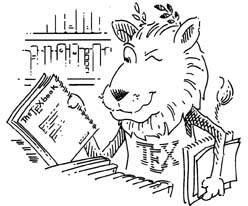
\includegraphics[width=\textwidth]{lion.png}
		\caption[SHORT LABEL]{A picture of a very handsome lion}
		\label{fig:figure1}
	\end{figure}





	
	
	\chapter{Conclusion}
	\label{chap:c}
	I hope this helps someone.  

Lots of the code was stolen with love from the UArk template.  Which, in turn, was stolen with love from UCSD.  I left comments which acted as signatures inside the .cls file to show some love to the original code authors and editors.  Please feel free to show me love when you steal this code for yourself.  This code is available for free, but feel free to buy me a beer some time.
	
	\bibliography{thesis}
	
	% Insert any appendices here
	\appendix
	\chapter{Sensor Board - Primary Circuit}
	\label{appendix:1}
	Your Appendix goes here.  Add more if you want.

	
	%% \chapter{Description of Research for Popular Publication}
% 
% \chapter{Executive Summary of Intellectual Property}
% This is a list of IP created. Consider both patent and commercialization.
% %what is latex for large format list like this? yeah- tabular. Set 1st colum skinny and 2nd column fat. I think it is auto.
% \begin{tabular}{cc}
% 	1.
% 	2.
% 	3.
% \end{tabular}
% 
% \chapter{Potential Patent and Commercialization Aspects of Listed Intellectual Property Items}
% \section{Patentability of Intellectual Property}
% %could each item be patented?
% \begin{tabular}{cc}
% 	1.
% 	2.
% 	3.
% \end{tabular}
% \section{Commercialization Prospects}
% %should each item be patented?
% 
% \begin{tabular}{cc}
% 	1.
% 	2.
% 	3.
% \end{tabular}
% \section{Possible Prior Disclosure of IP}
% The following items were discussed in a public forum or have published information that could impact the patentability of the listed IP.
% \begin{tabular}{cc}
% 	1.Pub 1
% 	2.UARK Poster Contest
% 	3.This Thesis... ha!
% \end{tabular}
% 
% \chapter{Broader Impacts of Research}
% \section{Applicability of Research Methods to Other Problems}
% %a paragraph of good size
% \section{Impact of Research Results on U.S. and Global Society}
% %paragraph of good size
% \section{Impact of Research Results on the Environment}
% %paragraph of good size
% 
% \chapter{Microsoft Project for MS MicroEP Degree Plan}
% %he has it on separate page - stupid?!?!??!?!
% %landscape, facing right
% 
% \chapter{Identification of All Software Used in Research and Thesis/Dissertation Generation}
% Computer \#1:\\
% Model Number: Dell Optiplex 780\\
% Serial Number: \\
% Location:\\
% Owner: Dr. So and So\\
% \begin{tabular}{ll}
% 	Software Name & Purchased By\\
% 	\hline
% 	Microsoft Windows 7 & \\
% 	TexWorks & Open Source\\
% 	MS Office 2010 & \\
% 	MS Project 2007 & \\
% 	Solid Works 2011 & \\
% 	Autocad 2011 Student Edition & \\
% \end{tabular}
% 
% Computer \#2:\\
% The laptop used for the microscope.
% Software: the program used to capture images
% 
% Computer \#3:\\
% 
% Computer \#4:\\
% 
% Computer \#5:\\
% 
% horizontal line here for signature, both\\
% %to be done
% Kyle Godin right hand side of page: Dr. Adam Huang
% 
% \chapter{All Publications Published, Submitted, and Planned}
% 
% \chapter{Plagiarism Check}
% This dissertation/ thesis was submitted by @name to http://www.turnitin.com for plagiarism reviewed by the TurnItIn company's software.  I examined the report on this dissertation that was returned by that plagiarism review site and attest that in my opinion the items highlighted by the software are incidental to common usage and are not plagiarized material.
% %need to fix this as well
% \vspace{1in}
% \makebox[1.5in]{\hrulefill}\\
% Ken Vickers\\
% Director, MicroEP Graduate Program\\
% \vspace{1in}
% \makebox[1.5in]{\hrulefill}\\
% @advisor\\
% Thesis Director\\

\begin{alwayssingle} %DO NOT touch this line.
	\okstatevita %DO NOT touch this line.
	\begin{addmargin}[.5in]{0pt} %DO NOT touch this line.
		\noindent Education: 
		\vspace{8pt}\\
		
		%% The syntax for the education command is:
		% \okvitaedu{Degree Title}{Degree Field}{Institution}{City}{State or Country}{Year}		
		\okvitaedu{Doctor of Philosophy}{Mathematics}{Oklahoma State University}{Stillwater}{Oklahoma}{May, 2017}
		\okvitaedu{Bachelor of Science}{Mathematics}{Oklahoma State University}{Stillwater}{Oklahoma}{2011}
		\noindent Experience:
		\vspace{8pt}\\
		%% The syntax for the experience command is:
		% \okvitaexp{Employer}{Position}{City}{State or Country}{Start date}{End date}

		\okvitaexp{Oklahoma State Univeristy}{Research/Teaching Assistant}{Stillwater}{Oklahoma}{August 2012}{date}
		\noindent Professional Memberships:
		\vspace{8pt}\\
		
		%% The syntax for the professional membership command is:
		% \okvitapro{Position (e.g. Member, Fellow, President, etc.)}{Organization}{Date of appointment}
		\okvitapro{President}{OSU Paddle People}{August, 2016}


%%%%%%%%%%%%%%%%%%%%%%%%%%%%%%%%%%%%%%%%%%%%%%%%%%%%%%%%%%
%%%                                                    %%%
%%%                     IMPORTANT!                     %%%
%%%                                                    %%%
%%%  The vita page should only be 1 page in length!!!  %%%
%%%                                                    %%%
%%%%%%%%%%%%%%%%%%%%%%%%%%%%%%%%%%%%%%%%%%%%%%%%%%%%%%%%%%










	\end{addmargin} %DO NOT touch this line.
	\vfill%DO NOT touch this line.
\end{alwayssingle} %DO NOT touch this line.
	
	
	
	
	
	
	
	
\end{document}